\documentclass[11pt]{article}
\usepackage[english]{babel}
\usepackage[utf8]{inputenc}
\usepackage[T1]{fontenc}
\usepackage{float}
\usepackage{lmodern,amsmath,amssymb,amstext,amsfonts,mathrsfs,graphicx,caption, subcaption}
\usepackage[width=14cm]{geometry}
\usepackage[colorlinks,pdfpagelabels,pdfstartview = FitV,bookmarksnumbered = true, bookmarksopenlevel=section, linkcolor = black,hypertexnames = false,citecolor = black,pdfpagelabels=false]{hyperref}
\usepackage{tablefootnote}
%\usepackage{rotating}
\usepackage{textcmds, enumitem}
\usepackage{sidecap} %, indentfirst
\usepackage[labelfont={bf,sf},font={small},labelsep=space]{caption}
\usepackage{chngcntr} % 			** Damit die Bilder Tabellen und Gleichungen 
\counterwithin{figure}{section}	%	** alle nach Kapiteln nummeriert sind.
\counterwithin{table}{section}%		**
\counterwithin{equation}{section}%	**	
\begin{document}
	
	\section{Methods}
	% Introduction.
	In this chapter, we will give an overview about the recurrent network (RNN) models for exploration of the feedforward recurrent alignment hypothesis that are evolved in this work. The firstly introduced symmetric network model builds the basis for modifications and extensions in other further models. The modified models will be introduced subsequently. Finally, we consider the role of learning could play in the feedforward recurrent alignment hypothesis. 
	
	\subsection{Symmetric Recurrent Network Model}
	% General Information about symmetric interaction network. 
	Due to the well understood mathematical characters of symmetric RNNs, they are often applied in models for neuroscience for a better understanding of certain dynamics.  
	Therefore, we firstly consider the basic case of having a symmetric recurrent network, which has a symmetric interaction matrix. For symmetric RNNs, if there is a connection between two neurons $n_i$ and $n_j$, the strength of the directed connection from the neuron $n_i$ to the neuron $n_j$ equals the directed connection from $n_j$ to $n_i$. 
	% A figure for network construction.
		\begin{figure}[H] 
			%\centering
			\begin{subfigure}[b]{0.4\textwidth}
				\centering
				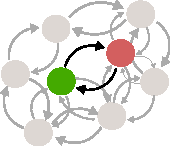
\includegraphics[width=0.2\textheight]{../figures/sym_net.pdf}
				\vspace{0.2cm}
				%\caption{Example of symmetric connections between two neurons.}
				\caption{}
			\end{subfigure}
			\hspace{0.4cm}
			\begin{subfigure}[b]{0.4\textwidth}
				\centering
				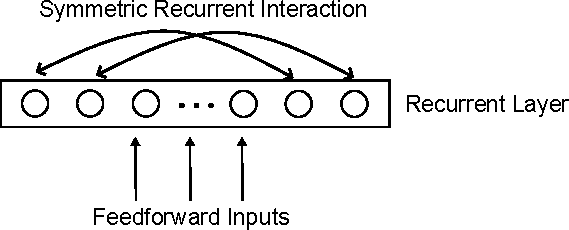
\includegraphics[width=0.4\textheight]{../figures/sym_recurrent.pdf}
				%\caption{Structure of a recurrent network (RNN)}
				\caption{}
			\end{subfigure}
		\caption{\textbf{Illustration of symmetric recurrent networks (symmetric RNNs).} \\ \textbf{(a)} An example of symmetric connections between two neurons in a network with multiple neurons. If there are connections between two neurons, here for example the green and red neurons, the directed connection from the green neuron to the red neuron has the same strength as the directed connection from the red to the green. \textbf{(b)} Structure of a symmetric RNN with feedforward inputs as the inputs for the recurrent layer. The connections between neurons inside the recurrent layer are symmetric, as illustrated in figure (a).}
		\label{fig:symmetric_RNN}
		\end{figure}
	
	\subsubsection{Symmetric Recurrent Interaction} \label{sec:symmetric_recurrent_interaction}
	% Definition of recurrent interaction. And how they constructed in the model.
	In the model, we consider a full rank real symmetric recurrent interaction matrix $J$ with Gaussian distributed entries with mean $0$ and variance $1$,
		\begin{equation} \label{eq:gaussian_distribution}
			{J_{ij}} \sim \mathcal{N}(0, 1).
		\end{equation}
	Besides, $J$ has full rank equals the number of neurons $n$ involved in the RNN, 
		\begin{equation}
			\text{rank} (J) = n \, , 
		\end{equation}
 	The eigenvalues of $J$ are limited by parameter $R < 1$ through normalization with the maximal original eigenvalue $\lambda_{\text{max}$ form $J$, 
		\begin{equation} \label{eq:eigval_normal}
			\tilde{\lambda_i} = \frac{R \lambda_i}{\lambda_{\text{max}}} \, \, \, \, \, \forall i \, ,
		\end{equation}
	where $\{\lambda_i\}_{i=1, ..., n}$ are the original eigenvalues of $J$ and $\{\tilde{\lambda_i}\}_{i = 1,...,n}$ the re-scaled eigenvalues. As a result, the maximal eigenvalues after the re-scaling would take value $R <1$.  
	
	\subsubsection{Response Steady State} \label{sec:steady_state_response_sym}
	
	\paragraph{Existence of Steady State}
	% Inputs and steady state output setting. Output dynamics. Stability analysis.
	
%	The feedforward input vectors $h \in \mathbb{R}^{n \times 1}$ for the RNN consists of two parts: the deterministic part $h_{\text{det}} \in \mathbb{R}^{n \times 1}$ and the stochastic part $h_{\text{stoch}} \in \mathbb{R}^{n \times 1}$. So, 
%		\begin{equation}
%			h = h_{\text{det}} + h_{\text{stoch}} . 
%		\end{equation}
%	The stochastic part 
	When considering the relationship between firing rate and synaptic current as linear, the dynamic system of the RNN illustrated in \ref{fig:symmetric_RNN} could be described as \cite{dayan2005theoretical}:
		\begin{equation} \label{eq:sym_response_ODE}
			\tau_r \frac{\mathrm{d} r}{\mathrm{d} t} = -r + J \cdot r + h \overset{\tau_r = 1}{\Rightarrow} \frac{\mathrm{d} r}{\mathrm{d} t} = -r + J \cdot r + h\, , 
		\end{equation}
	with the vector $r \in \mathbb{R}^{n \times 1}$ describing responses of neurons in the recurrent layer, the vector $h \in \mathbb{R}^{n \times 1}$ as feedforward inputs ,and $\tau_r$ the time constant controlling the speed of dynamic. 
	The steady state of the dynamic system \ref{eq:sym_response_ODE} can be received by setting the ordinary differential equation to zero. For simplicity, the time constant is set to one. We then have
		\begin{equation} \label{eq:steady_state}
			\frac{\mathrm{d} r}{\mathrm{d} t} = -r + J \cdot r + h = 0 \Rightarrow r = (I_n - J)^{-1} \cdot h =: r^* \, ,
		\end{equation}
	$r^*$ the steady state for responses. $I_n \in \mathbb{R}^{n \times n}$ is the identity matrix. Since $J$ is full rank, the matrix $(I_n - J)$ is invertible. Therefore, the steady state exists.
	
	\paragraph{Stability of Steady State}
	The dynamic \ref{eq:sym_response_ODE} could also be written in an elementary expression:
		\begin{equation}
			 f_i (r_1, ..., r_n) := \frac{\mathrm{d} r_i}{\mathrm{d} t} = - r_i + \sum_{j=1}^{n} J_{ij} r_j + h_i  \text{   for } i = 1, ..., n\, .
		\end{equation}
	The derivative of $f_i$ to $r_j$ is
		\begin{equation}
			\frac{\partial f_i}{\partial r_j} = 
			\begin{cases}
				-1 + J_{ij} & \text{if} \, \,  i = j \\
				J_{ij} & \text{if} \, \, i \neq j
			\end{cases} \, \, .
		\end{equation}
	The Jacobian matrix $A$ of the dynamic system $\frac{\mathrm{d} r}{\mathrm{d} t}$ is then
		\begin{equation} \label{eq:Jacobian_matrix}
			A := 
			 \begin{pmatrix}
				\dfrac{\partial f_1}{\partial x_1} & \cdots & \dfrac{\partial f_1}{\partial x_n}\\
				\vdots                             & \ddots & \vdots\\
				\dfrac{\partial f_n}{\partial x_1} & \cdots & \dfrac{\partial f_n}{\partial x_n}
			\end{pmatrix}
			= - I_n + J \, .
		\end{equation}
	Therefore, the Jacobian matrix $A$ is a linear transformation of the symmetric recurrent interaction matrix $J$, which is independent of the steady state response. So, $A$ has the same set of eigenvectors \footnote{For a symmetric matrix, the set of left eigenvectors equal the set of right eigenvectors} as $J$. With $E := \{e_i\}_{i = 1, ..., n}$ the matrix containing eigenvectors of $J$ column-wise, 
		\begin{equation} \label{eq:steady_state_eigenvalues_sym}
			(- I_n + J) E = - I_n \cdot E + J \cdot E = -I_n \cdot E + \Lambda \cdot E = (-I_n + \Lambda) E \, ,
		\end{equation}
	$\Lambda$ the diagonal matrix with eigenvalues $\{\lambda_i\}_{i = 1,...,n}$ of $J$ on its diagonal. This means, $\{-1 + \lambda_i\}_{i=1, ..., n}$ are eigenvalues for the Jacobian matrix A. 
	
	The eigenvalues of the Jacobian matrix $A$ determines the stability of steady states. Here, since the matrix $A$ is symmetric, all its eigenvalues $-1 + \lambda_i, i = 1, ..., n$ are from $\mathbb{R}$. Because the eigenvalues $\lambda_i$ of matrix $J$ is limited by the parameter $R<1$, defined in \ref{eq:eigval_normal}, we have 
		\begin{equation} \label{eq:sym_stable_fix_point}
			-1 + \lambda_i \overset{(\ref{eq:eigval_normal})}{<} -1 + 1 = 0 \, .
		\end{equation}
	That is, all eigenvalues of the Jacobian matrix $A$ are negative. This indicates that the steady state $r^*$ is stable. Under the assumption that the system reaches its steady state quick enough, we could apply the steady state $r^*$ for further analysis. 
	
	\subsubsection{Feedforward Recurrent Alignment for Symmetric Interactions} \label{sec:ffrec_definition}
	% TODO: The meaning of the feedforward recurrent alignment hypothesis (perhaps in the introduction better) 
	%In which case will it be applied.
	%TODO: The clarifying of mean firing rate in introduction perhaps?
	Generally, the feedforward inputs can be considered as a firing rate distribution with certain mean value. The mean firing rate is essential for the strength of inputs. We therefore consider mainly the mean firing rate of inputs. For the rest of work, if mentioning feedforward inputs without further definition, we mean the mean firing rate of inputs. 
	
	The alignment of a feedforward input $h \in \mathbb{R}^{n \times 1}$ with the recurrent network $J$ is defined as \cite{tragenap2023nature}
		\begin{equation} \label{eq:ffrec_align}
			\nu := \frac{h^T J h}{\parallel h \parallel_2 ^2}
		\end{equation}	
	If the inputs are aligned to the eigenvectors $e_i$ of the recurrent interaction $J$, i.e., 
		\begin{equation} \label{eq:h_prop_eigvec}
			h \propto e_i  \, ,
		\end{equation}
	the feedforward recurrent alignment $\nu$ is proportional to the eigenvalues $\lambda_i$, because inserting the proportionality (\ref{eq:h_prop_eigvec}) in (\ref{eq:ffrec_align}) leads to
		\begin{equation} \label{eq:ffrec_equals_eigval}
			\nu = \frac{h^T J h}{\parallel h \parallel_2 ^2} \propto \frac{{e_i}^T J e_i}{\parallel e_i \parallel_2 ^2} = \frac{\lambda_i {e_i}^T e_i}{\parallel e_i \parallel_2 ^2} = \lambda_i \, .
		\end{equation}
	It was therefore observed that the maximal alignment was attained when the input was proportional to the eigenvector $e_{\text{max}}$ with maximal eigenvalue $\lambda_{\text{max}}$ \cite{tragenap2023nature}. 
	
	\subsubsection{Response Properties for Evaluation} \label{sec:response_properties_for_evaluation}
	% TODO:general introduction where does this come? Or should it be in the introduction instead?
	% trial to trial correlation, intra-trial stability, dimensionality and alignment to spontaneous activity.
	\paragraph{Trial-to-trial correlation} \label{para:ttc_sym}
	Given the feedforward inputs that are from the same distribution for multiple trials, the correlation between responses from different trials indicates the reliability of the responses. Large correlation implies high reliability of the response generated by the RNN. 
	
	Model the inputs $h \in \mathbb{R} ^{n \times 1}$ as multivariate normal distributions with mean vector $\mu \in \mathbb{R}^{n \times 1}$ and covariance matrix $\Sigma \in \mathbb{R}^{n \times n}$
		\begin{equation} \label{eq:input_distribution}
			h \sim \mathcal{N} (\mu, \Sigma) \, \text{ with } \Sigma := \sigma_{\text{trial}}I_n. 
		\end{equation}
	Then, the steady state response $r^* = (I_n - J)^{-1} \cdot h $ from (\ref{eq:steady_state}) has the linearly transformed normal distribution
		\begin{equation} \label{eq:steady_state_distribute}
			r^* \sim \mathcal{N} \left((I_n - J)^{-1}\mu, (I_n - J)^{-1} \Sigma (I_n -J)^{-T}\right) \, ,
		\end{equation}
	where the mean vector and covariance matrix are linearly transformed. The property could be proved analogously as in \cite{Soch2019} with the moment-generating function of the multivariate normal distribution
		\begin{equation}
			M_h(t) = \mathbb{E}\left[\text{exp}(t^Th)\right] = \text{exp} \left[t^T \mu + \frac{1}{2} t^T \Sigma t \right] \, .
		\end{equation}
	Therefore, the moment-generating function of the random vector $r^*$ becomes
		\begin{equation}
			\begin{split}
				M_{r^*} & = M_h \left( (I_n-J)^{-T} t\right) \\
				        & = \text{exp} \left[
				         						t^T \left( (I_n - J)^{-1} \mu\right) + \frac{1}{2} t^T (I_n - J)^{-1} \Sigma (I_n - J)^{-T} t    
				         				\right]
			\end{split} \, ,
		\end{equation}
	which indicates the linearly transformed distribution of $r^*$ as in (\ref{eq:steady_state_distribute}).
	
	As calculated in \cite{tragenap2023nature}, the trial to trial correlation $\beta$ for one stimulus $s$ is calculated by taking the mean of correlations between $N$ response trials that evoked by this stimulus. That is
		\begin{equation} \label{eq:ttc_sym}
			\beta_s = \frac{2}{N(N-1)} \sum_{i = 1, j = i+1}^{N} corr(r_i^s, r_j^s) \, ,
		\end{equation}
	where $r_i^s$ is the $i$-th response trial that evoked by stimulus $s$. 
	
	\paragraph{Intra-trial stability}
	
	It was observed that presenting ongoing visual grating stimuli, the responses in the visually naive cortex has a stronger variation than they are after visual experience. In order to reflect the variation of responses during the stimulation period, the quantity of "intra-trial stability" was defined \cite{tragenap2023nature}. 
	
	To model the time dependent input $h(t) \in \mathbb{R}^{n \times 1}$ distributed as (\ref{eq:input_distribution}) and its evoked steady state responses $r(t) \in \mathbb{R}^{n \times 1}$, the following stochastic differential equations were formulated
		\begin{subequations} \label{eq:sde_intra_trial_stability}
			\begin{align}
				\mathrm{d} h & = \mu \mathrm{dt} + \sigma_{\text{time}} \mathrm{d} W \\
				\mathrm{d} r & = (-r + J \cdot \mu) \mathrm{d}t + \sigma_{\text{time}} \mathrm{d} W \, ,
			\end{align}
		\end{subequations}
	with $W$ the Wiener process, which is a continuous-time stochastic process with independent Gaussian increments. 
	
	To approximate the evoked response $r(t)$, the equation (\ref{eq:sde_intra_trial_stability}b) is solved numerically with Euler-Maruyama scheme 
		\begin{equation} \label{eq:euler_maruyama}
			r_{t+1} = r_t + (-r_t + J \cdot \mu) \Delta t + \sigma_{\text{time}} \sqrt{\Delta t} \Delta \tilde{W}_t \, ,
		\end{equation}
	with $r_t$ the response at time point $t$, $\Delta t$ the step width for iteration, and $\Delta \tilde{W}_t \in \mathbb{R}^{n \times 1}$ the Gaussian increment at time point $t$ defined as the multivariate normal distribution with mean vector $0_v$ and covariance matrix $I_n$
		\begin{equation}
			\Delta \tilde{W}_t \sim \mathcal{N}(0_v, I_n) \, .
		\end{equation}
	
	For a certain step width $\tilde{\Delta t}$, the intra-trial stability $c(\Delta \tilde{t})$ was defined by the correlation between normalized response at time $t$ and its delayed response at time $t + \Delta \tilde{t}$ 
		\begin{equation}
			c(t, \Delta \tilde{t}) := \bar{r}(t)^T \bar{r}(t + \Delta t) \, , 
		\end{equation}
	where the normalized response is defined as
		\begin{equation}
			\bar{r}(t) := \frac{r - \langle r \rangle}{\sigma_r} \, ,
		\end{equation}
	with mean value of $r$ denoted by $\langle r \rangle$ and standard deviation by $\sigma_r$. 
	
	The final intra-trial stability for a time period $T$ is the time-averaged value over all time points $0 \leq t \leq T - \Delta \tilde{t}$
		\begin{equation} \label{eq:its_sym}
			\begin{split}
				\bar{c}{(\Delta \tilde{t})} &= \frac{1}{T-\Delta \tilde{t}} \int_{0}^{T-\Delta \tilde{t}} c(t, \Delta \tilde{t}) \mathrm{d} t\\
				                            &= \frac{1}{T-\Delta \tilde{t}} \int_{0}^{T-\Delta \tilde{t}} \bar{r}(t)^T \bar{r}(t + \Delta t) \mathrm{d} t \, .
			\end{split} 
		\end{equation}
	
	\paragraph{Dimensionality}
	%TODO: Sources for dimensionality meaning and linear dimensionality definition.
	
	The dimensionality of neuron responses reflect the complexity of the informatbetaion they encoded. %TODO: literature.
	A diverse response pattern corresponds with a broader distribution of the variance over principal components, leading to a higher-dimensional linear manifold. %TODO: lietrature
	The corresponding dimensionality for more diverse and variable response pattern is therefore higher \cite{tragenap2023nature}. %TODO: Is the understanding correct? Further literatures?
	Given the multivariate normal distributed inputs $h \in \mathbb{R}^{n \times 1}$
		\begin{equation} \label{eq:input_distribution_dimensionality}
			h \sim \mathcal{N}(0_v, \Sigma^{\text{Dim}}) \, ,
		\end{equation}
	the linear transformed responses (analogously as (\ref{eq:steady_state_distribute})) are
		\begin{equation} \label{eq:response_distribution_dimensionality}
			r \sim \mathcal{N}(0_v, (I_n - J)^{-1} \Sigma^{\text{Dim}} (I_n - J)^{-T})
		\end{equation}
	with 
		\begin{equation} \label{eq:Sigma_dim}
			\Sigma^{\text{Dim}} := \sum_{i=L}^{L+M} \text{exp}\left(\frac{-2(i-L)}{\beta}\right) e_i e_i^T \, , 
		\end{equation}
	in which the parameter $M := \kappa \beta$ and $\beta$ reflects the dimensionality \cite{tragenap2023nature} and $\kappa$ for determining the number of directions $e_i$ that contribute to the dimensionality. Since the eigenvectors of $J$ build a set of basis for $\mathbb{R}^n$, they could be chosen as $e_i$ for (\ref{eq:Sigma_dim}). Hereby, the eigenvectors are ordered according to their eigenvalues in descending order. The exponential factor in (\ref{eq:Sigma_dim}) simulates the exponential decay of variance ratio observed in prior data \cite{tragenap2023nature}. 
	
	The linear effective dimensionality based on participation ratio was defined %TODO: literature
	to quantify the tendency of dimensionality during visual maturation.
	The participation ratio is defined as %TODO: literature.
		\begin{equation} \label{eq:effective_dimensionality_analytical}
			d_{\text{eff}} := \frac{\left(\sum_{i} \lambda_i\right)^2}{\left( \sum_{i} \lambda_i^2\right)} \, ,
		\end{equation}
	where $\lambda_i$ the eigenvalues of a certain response pattern with covariance $\mathbf{\Sigma}$. Since as defined in (\ref{eq:Sigma_dim}), $\Sigma^{\text{Dim}}$ has the same eigenvectors (aka. principal components )as $J$. Therefore, the eigenvalues $\lambda_i^{\text{Dim}}$(aka. variance ratio or variance explained) for $\Sigma^{\text{Dim}}$ are transformed eigenvalues $\lambda_i$ of $J$ expressed as
		\begin{equation}
			\lambda_i^{\text{Dim}} = \text{exp}\left(\frac{-2(i-L)}{\beta}\right) \lambda_i \, .
		\end{equation}
	The covariance of the responses share the same eigenvectors as $\Sigma^{\text{Dim}}$ based on its distribution (\ref{eq:response_distribution_dimensionality}) and therefore also the same as $J$. The eigenvalues (aka. variance ratio) for the responses could be constructed analogously with
		\begin{equation} \label{eq:response_variance_ratio_dimensionality}
			\lambda_i^{\text{Act}} = \text{exp}\left(\frac{-2(i-L)}{\beta}\right) \frac{1}{(1-\lambda_i)^2} \, ,
		\end{equation}
	for $i = L, ..., L+M$, due to the inverse transformation. 
%	 For the covariance $\Sigma^{\text{Dim}}$ from inputs, if having its eigenvalues $\lambda_i^{\text{Dim}}$, the eigenvalues $\lambda_i^{\text{Act}}$ of the steady state responses could be transformed based on the distribution (\ref{eq:response_distribution_dimensionality}). It leads to the following relation
%		\begin{equation}
%			\lambda_i^{\text{Act}} = \frac{1}{(1-\lambda_i^{\text{Dim}})^2} = \, . %TODO: the exp factors
%		\end{equation}
%	Therefore, the 
	
	Insert the eigenvalues of responses (\ref{eq:response_variance_ratio_dimensionality}) in the formula for effective dimensionality to get the final formulation of dimensionality for responses
		\begin{equation} \label{eq:dim_analytical_sym}
			d^r_{\text{eff}} = \frac{\left(\sum_{i = L}^{L + M} \text{exp}\left(-2 \frac{i-L}{\beta}\right)(1-\lambda_i)^{-2}\right)^2}{\sum_{i=L}^{L+M} \text{exp}\left(-4 \frac{i-L}{\beta}\right)(1-\lambda_i)^{-4}}
		\end{equation}
	
	Since the vector of explained variance ratios in the principal component analysis (PCA) is the normalized vector containing eigenvales of the covariance matrix re-scaled by the largest eigenvalue in descending order, which then explains how much variance does the corresponding principal component contribute. Therefore, another way to access the dimensionality is to empirically determine the explained ratio of generated data samples through PCA and insert the variance ratio into the definition of effective dimentionality, i.e.,
		\begin{equation} \label{eq:dim_empirical_sym}
			d_{\text{eff}} = \frac{\left(\sum_{i=L}^{L+M}\text{var}_i\right)^2}{\sum_{i=L}^{L+M}\text{var}_i^2} 
		\end{equation}
	with $\text{var}_i$ the $i$-th variance ratio. 
	
	\paragraph{Alignment with spontaneous activity}
	
	The alignment of activity patterns to spontaneous activity reflects in principle the size of overlaps between activity patterns and spontaneous activity pattern. 
	% is in principle the dimensionality explained by the principal components of spontaneous activity. 
	Assuming having the evoked response pattern as $R$ and the spontaneous activity pattern as $S$, the projection of $R$ to $S$ could be quantified as the covariance matrix of $R$ explained by the principal components (a.k.a. eigenvectors of covariance matrix) of $S$, which results a variance ratio vector
	%we then have the variance of activity pattern $R$ explained by principal components of pattern $S$ expressed as a vector $\mathbf{v}$ with 
		\begin{equation} \label{eq:var_explain_spont_act_sym}
			\mathbf{v}_i = \frac{\mathbf{p}_{i, S}^T \cdot \mathbf{\Sigma_R} \cdot \mathbf{p}_{i, S}}{\text{Tr}(\mathbf{\Sigma_R})} \, , 
		\end{equation}
	for $i = 1, ..., n$. $\mathbf{p}_{i, S}$ are the principal component of spontaneous activity and $\mathbf{\Sigma_R}$ the covariance matrix of evoked activity. 
	%TODO: the connections between variance explained and alignment. 
	%It was observed in \cite{tragenap2023nature} that patterned visual experience is required to cause stable alignment between visual responses and the spontaneous activities, while naive visual responses show only loose alignment with spontaneous activities. To capture this change of property as a quantity instead of a vector as (\ref{label}), it had to firstly define the alignment between two activity patterns. The alignment of $R$ to $S$ was defined as the average of pattern $S$ explained by normalized trials $r_{i, R}$. The alignment between pattern $S$ and one trial $r_{i, R}$ from $R$ is defined as
	Consider the projection of activity pattern $R$ in all directions of spontaneous pattern $S$ together to reflect the overall overlaps between two patterns, we calculate firstly the alignment between a response trial $r_{i, R}$ form $R$ to the spontaneous pattern $S$ 
		\begin{equation} \label{eq:align_to_spont_act_sym}
			\gamma_i = \frac{r^T_{i, R} \cdot \Sigma_S \cdot r_{i,R}}{\Vert r_{i, R} \Vert^2 \text{Tr}(\Sigma_S)}\, ,
		\end{equation}
	where $\Sigma_S$ is the covariance of pattern $S$. The final alignment between $S$ and $R$ is then the average value of alignment between $S$ and all trials of $R$. 
	
	To model the inputs and responses, we assumed that spontaneous activity was evoked by inputs from broad sources. Besides, since the spontaneous activity already exists almost a week before eye opening, we assume that they already fit to the activity space generated by recurrent network \cite{tragenap2023nature}. Therefore, the inputs would be explained by more directions (or eigenvectors) than stimuli evoked responses as modeled before with (\ref{eq:input_distribution_dimensionality}), that is higher dimensionality. Since the parameter $\beta$ in (\ref{eq:input_distribution_dimensionality}) indicates the dimensionality, we could set for spontaneous activity higher $\beta_{\text{spont}} > \beta$ to generate high dimensional inputs. 
	Therefor, we than have the broad inputs $h^{\text{spont}} \in \mathbb{R}^{n \times 1}$ and spontaneous activity $r^{\text{spont}} \in \mathbb{R}^{n \time 1}$, which are multivariate distributed vectors 
		\begin{equation}
			\mathbf{h}^{\text{spont}} \sim \mathbf{\mathcal{N}}(\mathbf{0_v}, \mathbf{\Sigma}^{\text{spont}})
		\end{equation}
	and 
		\begin{equation}
			\mathbf{r}^{\text{spont}} \sim \mathbf{\mathcal{N}}\left( \mathbf{0_v}, (\mathbf{I_n} - \mathbf{J})^{-1} \mathbf{\Sigma}^{\text{spont}}(\mathbf{I_n} - \mathbf{J})^{-T}\right) \, .
		\end{equation}
	The covariance matrix $\mathbf{\Sigma}^{\text{spont}}$ is constructed in the same way as $\mathbf{\Sigma}^{\text{Dim}}$ only with $L=1$ and larger $\beta_{\text{spont}}$, that is
		\begin{equation} \label{eq:Sigma_spont}
			\mathbf{\Sigma}^{\text{spont}} := \sum_{i=1}^{M+1} \text{exp}\left(\frac{-2(i-1)}{\beta_{\text{spont}}}\right) e_i e_i^T \, .
		\end{equation}
	
	\clearpage
	\subsection{Asymmetric Recurrent Network Model}
	% Reason for considering asymmetric networks.
	Different as symmetric recurrent networks, asymmetric recurrent networks do not necessary have symmetric interaction strength between two neurons. That is, if we have two neurons $n_i$ and $n_j$, the interaction strength from $n_i$ to $n_j$ can generally differ from the interaction strength from $n_j$ to $n_i$. Therefore, the network has a more complex neural interactions and dynamics. Compare to symmetric recurrent network, the asymmetric recurrent network reflects more general neural interactions and thus more biologically realistic. 
	
	\begin{figure}[H] 
		%\centering
		\begin{subfigure}[b]{0.4\textwidth}
			\centering
			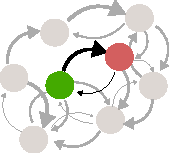
\includegraphics[width=0.2\textheight]{../figures/asym_net.pdf}
			\vspace{0.2cm}
			%\caption{Example of symmetric connections between two neurons.}
			\caption{}
		\end{subfigure}
		\hspace{0.4cm}
		\begin{subfigure}[b]{0.4\textwidth}
			\centering
			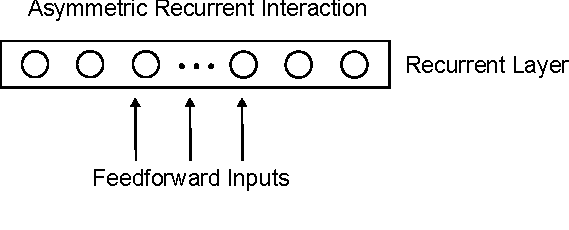
\includegraphics[width=0.4\textheight]{../figures/asym_recurrent.pdf}
			%\caption{Structure of a recurrent network (RNN)}
			\caption{}
		\end{subfigure}
		\caption{\textbf{Illustration of asymmetric recurrent networks (asymmetric RNNs).} In general, asymmetric recurrent networks do not have symmetric interaction strength between to neurons. \textbf{(a)} An example of asymmetric connections between two neurons in a network with multiple neurons. There are connections between the green and red neurons. The connection from green one to red one is stronger than the connection from the red to green. There are also connections that only from one neuron to the other but no connection back from the other neuron.  \textbf{(b)} Structure of a asymmetric RNN with feedforward inputs as the inputs for the recurrent layer. The connections between neurons inside the recurrent layer are asymmetric, as illustrated in figure (a).}
		\label{fig:asymmetric_RNN}
	\end{figure}
	
	 
	\subsubsection{Asymmetric Recurrent Interaction} \label{sec:asym_recurrent_network}
	% Definition of the asymmetric recurrent interaction network. The problems that come up with the asymmetricity.
	For the modeling, we construct the asymmetric interaction matrix $J$ through disturbing symmetric interaction matrix by a general asymmetric random matrix
		\begin{equation} \label{eq:asym_interaction_matrix}
			J = a J_{\text{sym}} + (1-a) J_{\text{asym}} \, .
		\end{equation}
	The symmetric part is generated as described in section \ref{sec:symmetric_recurrent_interaction}. The asymmetric part has also Gaussian distributed entries with mean $0$ and $1$ as variance (\ref{eq:gaussian_distribution}). Parameter $a$ therefore indicates the degree of symmetry in the network. 
	
	The recurrent network dynamics remains the same as in symmetric case, described by (\ref{eq:sym_response_ODE}). Therefore, the steady state also keeps its form as (\ref{eq:steady_state}). Stability analysis of the steady state follows the same procedure as for symmetric interaction matrix (section \ref{sec:steady_state_response_sym}). However, here we have to mind that the asymmetric interaction matrix $J$ now have left and right eigenvectors, which are not identical to each other any more. The Jacobian matrix $A = -I_n + J$ defined from (\ref{eq:Jacobian_matrix}) still has the same set of eigenvectors as $J$. The eigenvalues are found in the similar way as (\ref{eq:steady_state_eigenvalues_sym}) but with left and right eigenvectors. If $E_l$ and $E_r$ the matrices containing the left and right eigenvectors column-wise, it follows
		\begin{equation}
			\begin{split}
				E_l^*(-I_n + J) &= - E_l^* + E_l^* J =  - E_l^* + \Lambda E_l^* = (-I_n + \Lambda) E_l^* \\
				(-I_n + J) E_r &= - E_r + J E_r = -E_r + E_r \Lambda = E_r (-I_n + \Lambda) \, , 
			\end{split}
		\end{equation}	
	with $E_l^*$ the conjugate transport matrix of $E_l$, $I_n$ the identity matrix, and $\Lambda$ the diagonal matrix that contains eigenvalues of $J$ on its diagonal. The eigenvalues $\{\lambda_i\}$ for $J$ are in general complex numbers
	\begin{equation}
		\{\lambda_i \in \mathbb{C} \mid \lambda_i \text{ eigenvalues of $J$}\} \, .
	\end{equation}
	Therefore, the eigenvalues for the Jacobian matrix $A$ is now $-I_n + \Lambda \in \mathbb{C}^{n \times n}$. 
	
	To determine the stability of steady state, we now have to consider the real part of $(-I_n + \Lambda)$. If $\exists i: -1 + \text{Re}(\lambda_i) > 0$, the steady state will be unstable. However, if $\forall i: -1 + \text{Re}(\lambda_i) < 0$, the steady state is then stable and we will have
		\begin{equation} \label{eq:asym_stable_fix_point}
			\forall i: -1 + \text{Re}(\lambda_i) < 0 \, \,  \Rightarrow \, \, \text{lim}_{t \rightarrow \infty} r(t) = r^*
		\end{equation}
	Thus, we need to limit the range of eigenvalues for $J$ such that the real part of eigenvalues is limited by $R < 1$. The limitation could be achieved by dividing the complex eigenvalues by maximal absolute magnitude.
		\begin{equation} \label{eq:asym_normalization}
			\tilde{\lambda}_i = \frac{R \lambda_i}{\Vert\lambda\Vert_{\text{max}}} \, \, \, \, \, \forall i \, ,
		\end{equation}  
	The contribution of eigenvalues is influenced by the parameter $a$, which determines the proportion of symmetric interaction. In the case of only having symmetric interaction network, all eigenvalues are real and therefore the distribution forms a line in the complex plane. On the other hand, if $J$ is only a general asymmetric interaction network, the distribution forms a circle \cite{rajan2006eigenvalue}. For $a$ between $0$ and $1$, the distribution is a symmetric ellipse. 
		\begin{figure} [H]
			\centering
			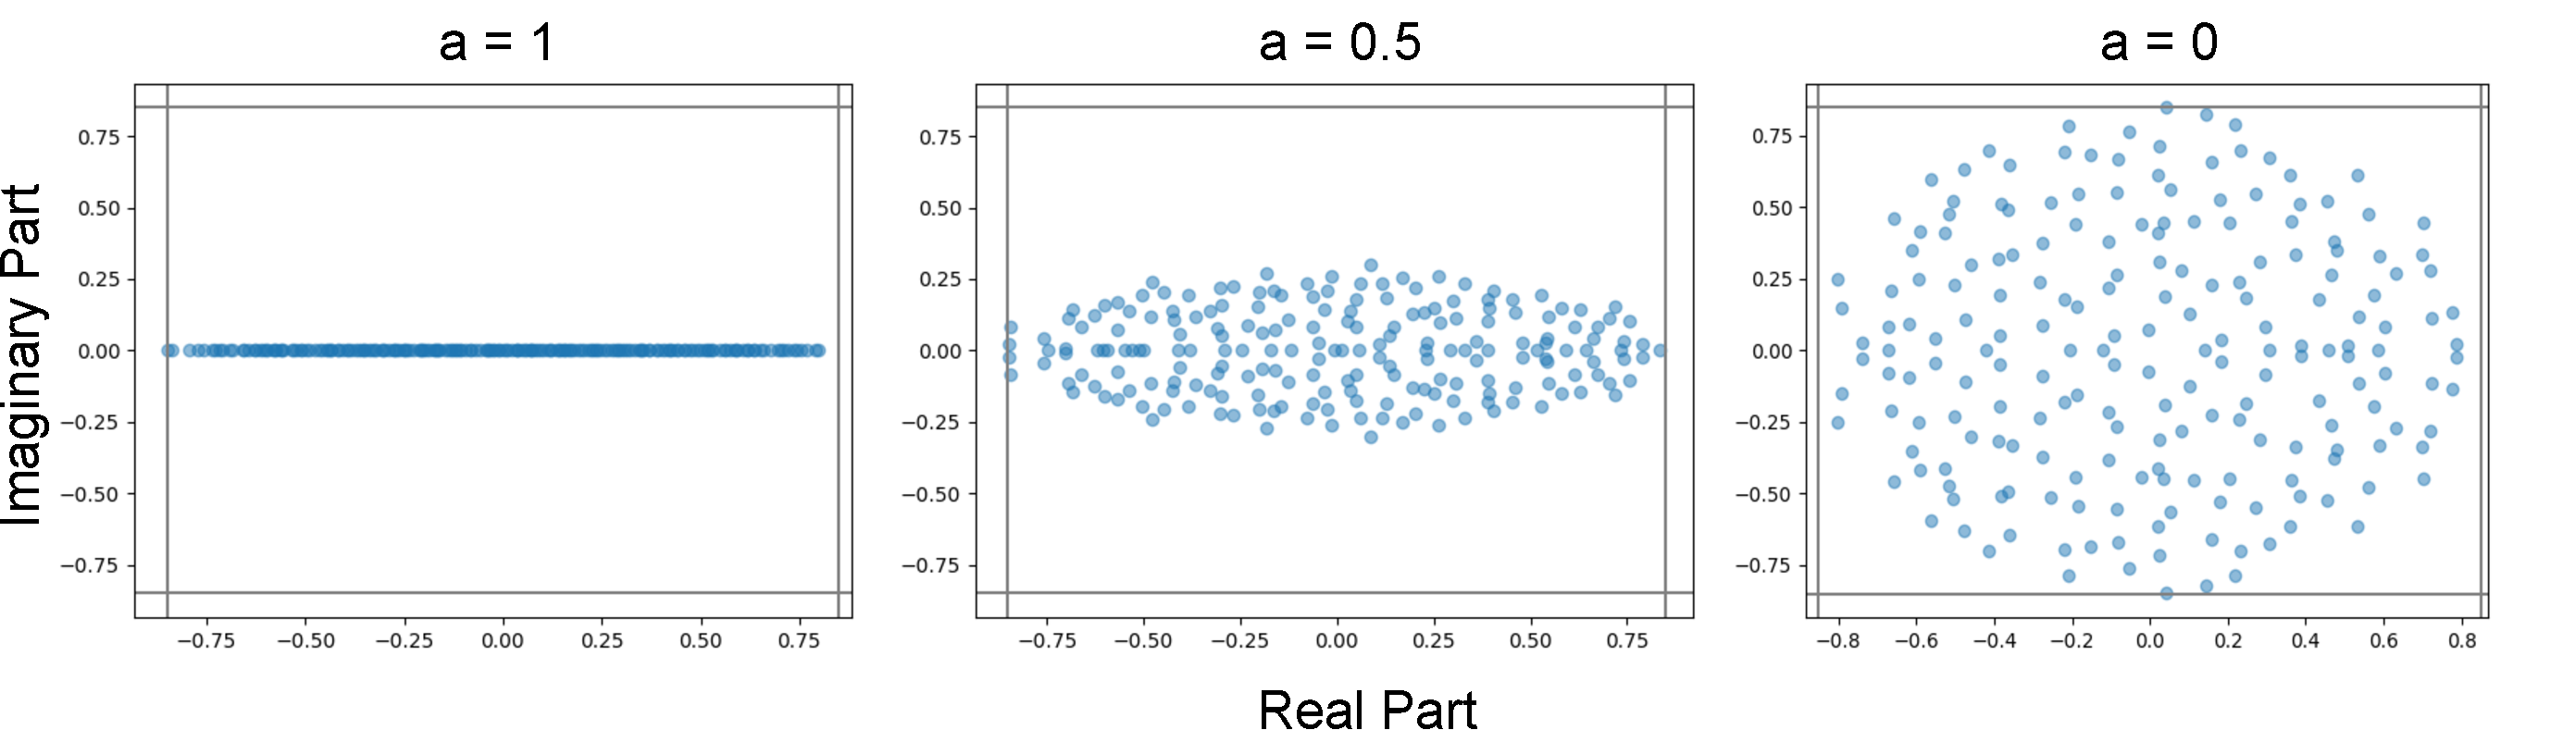
\includegraphics[width=\textwidth]{../figures/asym_eigval_distribution.pdf}
			\caption{\textbf{Eigenvalue distribution in dependence of parameter $a$ in (\ref{eq:asym_interaction_matrix}).} In general, an asymmetric matrix has eigenvalues in complex plane. The degree of symmetry determines the form of distribution from a line ($a = 1$, only real eigenvalues) to a full circle ($a = 0$) with radius $R < 1$. Between $a = 0$ and $a = 1$, the distribution is a symmetric ellipse along imaginary part $=0$. Sub figures from left to right show the eigenvalue distribution in the complex plane from $a = 1, 0.5,$ and $1$. The gray line marks the radius $-R$ and $R$. Here $R = 0.85 < 1$.}
		\end{figure}
	
	\subsubsection{Modifications of Feedforward Recurrent Alignment for Asymmetric Interactions} \label{sec:modify_ffrec_alignment_score}
	% Reason for modification.
	% The three Hypothesis/Modification that were looked at. 
	We want to have the similar quantification of feedforward recurrent alignment as for the symmetric interaction matrix (section \ref{sec:ffrec_definition}). However, when aligning the feedforward input to eigenvectors of asymmetric recurrent interaction network $J$ like (\ref{eq:ffrec_equals_eigval}), the result calculated by (\ref{eq:ffrec_align}) is a complex number and can therefore be hardly interpreted. To embed such a sore with analogical idea, we deliberate the following modifications and try to discover the outcomes. 
	
	Aligning feedforward input $h \in \mathbb{C}^{n \times 1}$ to the asymmetric interaction $J$, we consider:
		\begin{enumerate}
			\item \label{sec:modicication_real_part} Only the real part of input $h$ and calculate the feedforward recurrent alignment with $\tilde{h} = \text{Re}(h) \in \mathbb{R}^{n \times 1}$.
				\begin{equation} \label{eq:ffrec_real_part}
					\nu_{\text{Re}} := \frac{\tilde{h}^T J \tilde{h}}{\Vert \tilde{h} \Vert^2} = \frac{\text{Re}(h)^T J \text{Re}(h)}{\Vert \text{Re}(h)\Vert^2} \, .
				\end{equation}
			\item \label{sec:modification_magnitude} Consider the magnitude of all entries in feedforward input $h$ and take $\tilde{h_i} = \vert h_i \vert \in \mathbb{R} \, \, \forall i$. Therefore $\tilde{h} \in \mathbb{R}^{n \times 1}$.
				\begin{equation} \label{eq:ffrec_mag}
					\nu_{\text{mag}} := \frac{\tilde{h}^T J \tilde{h}}{\Vert \tilde{h} \Vert^2} \text{ with } \tilde{h}_i = \vert h_i \vert \in \mathbb{R} \, .
				\end{equation}
			\item \label{sec:modification_symmetrized} Symmetrize $J$ through
				\begin{equation} \label{eq:symmetrized_J}
					\tilde{J} = \frac{J + J^T}{2} \, .
				\end{equation}
				Instead of align the feedforward input directly to $J$, we align indirectly to $\tilde{J}$ with its eigenvectors $\tilde{e}_i \in \mathbb{R}^{n \times 1}$. If having feedforward input aligned to eigenvectors to $J$ with $\tilde{h} = \tilde{e}_i $, the feedforward recurrent alignment will be calculated with eigenvectors of $\tilde{J}$ instead:
				\begin{equation} \label{eq:ffrec_symmetrized}
					\nu_{\text{sym}} =  \frac{\tilde{h}^T J \tilde{h}}{\Vert \tilde{h} \Vert^2} = \frac{\tilde{e}_i^T J \tilde{e}_i}{\Vert \tilde{e}_i \Vert^2} \in \mathbb{R} \, ,
				\end{equation}
				with $\tilde{\lambda}_i$ eigenvalues of $\tilde{J}$ . 
		\end{enumerate}
	
	\subsubsection{Related Modification for Evaluation} \label{sec:modification_asym}
	% Change in dimensionality 
	As for symmetric interaction network, four activity properties are taken into account to evaluate the feedforward recurrent alignment hypothesis with measurement of the alignment scores. In the case of asymmetric interaction, the modified alignment scores (section \ref{sec:modify_ffrec_alignment_score}). 
	
	More than the four response properties that considered in the case of symmetric recurrent interaction matrix, for new definition of feedforward recurrent alignment scores, the monotony of score and corresponding eigenvalues have to be verified. Following are more details about how modifications in section \ref{sec:modify_ffrec_alignment_score} influence the modulation of properties that are involved in the evaluation. 
	
	\paragraph{Monotony} For a certain eigenvector $e_i$, its corresponding eigenvalues $\lambda_i$ can reflect the strength of response due to the response amplification %TODO: response amplification in methods!!. 
	Dominant eigenvectors with large eigenvalues can therefore trigger strong response and suppress noise, leading to more reliable evoked activity. If the feedforward recurrent alignment score could well predict the reliability of evoked activities, inserting dominant eigenvectors should result in large score value. Therefore, large feedforward recurrent alignment score calculated with modified eigenvectors $\tilde{h}$ should corresponds with large eigenvalue. In other words, a monotonic positive correlation should exist between eigenvalues and feedforward recurrent alignment score inserting corresponding modified eigenvectors. 
	
		
	\paragraph{Trial-to-trial correlation} 
	Similar to the case with symmetric interaction network, the first characteristic that is evaluated is the trial-to-trial correlation. With above modifications in section \ref{sec:modify_ffrec_alignment_score}, the inputs are aligned to $\tilde{h}$ for all modifications. That is the mean vector for modeling the inputs by multivariate normal distribution is determined by $\tilde{h}$. 
		\begin{equation}
				h \sim \mathcal{N}(\tilde{h}, \sigma_{\text{trial}I_n}) \, .
		\end{equation}
		The steady state response evoked by the inputs are transformed multivariate normal distribution
		\begin{equation}
				r \sim \mathcal{N}\left((1-J)^{-1}\tilde{h}, \sigma_{\text{trial}} (1-J)^{-1} (1-J)^{-T}\right) \, .
		\end{equation}
	Trial-to-trial correlation is determined by $\beta_s$ defined in equation (\ref{eq:ttc_sym}). 
	
	\paragraph{Intra-trial stability} Modulation of the single trial is described by the stochastic differential equations (\ref{eq:sde_intra_trial_stability}). When the inputs are aligned to the modified eigenvectors, the mean value of inputs are again determined by $\tilde{h}$ defined in modifications above. As a result, the stochastic differential equations after modification is 
		\begin{subequations}
			\begin{align}
				\mathrm{d} h & = \tilde{h} \mathrm{dt} + \sigma_{\text{time}} \mathrm{d} W \\
				\mathrm{d} r & = (-r + J \cdot \tilde{h}) \mathrm{d}t + \sigma_{\text{time}} \mathrm{d} W \, ,
			\end{align}
		\end{subequations}
	The solution of evoked activity is followed by Euler-Maruyama scheme (\ref{eq:euler_maruyama}). Intra-trial stability is then calculated with (\ref{eq:its_sym}). 
	
	\paragraph{Dimensionality}% Modification for the covariance matrix and analytical dimensionality. 
	With symmetric interaction networks, the covariance matrix for generation of inputs and responses is constructed with eigenvectors of interaction matrix since they build up a set of basis for $\mathbb{R}^{n \times n}$. But with asymmetric interaction matrix, the eigenvectors are basis for $\mathbb{C}^{n \times n}$. If using complex eigenvectors, the inputs and responses will be complex without plausible interpretations. Therefore, the construction of the covariance matrix need to be modified synchronously to have at least vectors from $\mathbb{R}^{n \times 1}$. 
				  
	The same problem exists also for the analytical calculation for effective dimensionality (\ref{eq:effective_dimensionality_analytical}): we now have complex eigenvalues that lead to the dimensionality also complex. To overcome this problem, we work along the same modifications as above for covariance matrix.
				  
	As a result, having $e_i$ eigenvectors and $\lambda_i$ of asymmetric interaction network $J$
	  \begin{itemize}
			  	\item For modification \ref{sec:modicication_real_part} (\ref{eq:ffrec_real_part}), applying $\tilde{e}_i = \text{Re}(e_i)$ for construction covariance matrix and $\tilde{\lambda}_i = \text{Re}\lambda_i$ for calculation of effective dimensionality. 
			  	\item For modification \ref{sec:modification_magnitude} (\ref{eq:ffrec_mag}), applying magnitude for all entries in $e_i$ to formulate $\tilde{e}_i$ and $\tilde{\lambda}_i = \vert \lambda_i \vert$ also magnitude of eigenvalues. 
			  	\item For modification \ref{sec:modification_symmetrized} (\ref{eq:ffrec_symmetrized}), applying eigenvectors $\tilde{e}_i$ and eigenvalues $\tilde{\lambda}_i$ from $\tilde{J}$ (\ref{eq:symmetrized_J}).
	  \end{itemize}
			  		
  	 The covariance matrix for generating inputs is constructed similar to it with symmetric interaction network (\ref{eq:Sigma_dim}) but with $\tilde{e}_i$ defined above, 
  	  	\begin{equation} \label{eq:modifications_dim}
  	  		\Sigma^{\text{Dim}} := \sum_{i=L}^{L+M} \text{exp}\left(\frac{2(i-L)}{\beta}\right) \tilde{e}_i \tilde{e}_i^T \, .
  	  	\end{equation}
		  	  	
 	  Analogously, calculating the effective dimensionality defined by (\ref{eq:dim_analytical_sym}) but with $\tilde{\lambda}_i$,
  	  	  	\begin{equation} \label{eq:modification_eff_dim}
  	  	  		d^r_{\text{eff}} = \frac{\left(\sum_{i = L}^{L + M} \text{exp}\left(-2 \frac{i-L}{\beta}\right)(1-\tilde{\lambda}_i)^{-2}\right)^2}{\sum_{i=L}^{L+M} \text{exp}\left(-4 \frac{i-L}{\beta}\right)(1-\tilde{\lambda}_i)^{-4}}
  	  	  	\end{equation}
		  	  	
	\paragraph{Alignment to spontaneous activity}. % Modification due to dimensionality modification.
	Since the same formulation of covariance matrix with a larger parameter $\beta_{\text{spont}}$ is used for generation of broader endogenous inputs, the same modifications above for dimensionality (\ref{eq:modifications_dim}) can be taken over into covariance matrix of endogenous inputs like (\ref{eq:Sigma_spont}),
	  	\begin{equation} \label{eq:Sigma_spont_asym}
	  		\Sigma^{\text{spont}} := \sum_{i=1}^{\kappa\beta_{\text{spont}}} 		\text{exp}\left(\frac{2(i-1)}{\beta_{\text{spont}}}\right) \tilde{e}_i \tilde{e}_i^T \, .
	  	\end{equation}
				  
	\clearpage
	\subsection{Low Rank Recurrent Network Model}
	% Reasons and importance for looking at low rank networks. (limitations of full rank RNN and advantages of low-rank RNN.)
	Until now, we considered full ranked random recurrent networks in both symmetric and asymmetric cases. Those fully recurrent connectivity structure is one of the most popular and best-studied classes of network models. However, randomly connected network display only very stereotyped responses to external inputs, can implement only a limited range of iniput-output computations \cite{mastrogiuseppe2018linking}. 
	
	Furthermore, experimental large-scale neural recordings have established that the transformation of sensory stimuli into motor outputs relies on low-dimensional dynamics at the population level \cite{mastrogiuseppe2018linking}. Besides, actual cortical connectivity appears to be neither fully random nor fully structured \cite{harris2013cortical}. Understanding how low-dimensional computations on mixed, distributed representations emerge from the structure of the recurrent connectivity and inputs to cortical networks is a major challenge \cite{mastrogiuseppe2018linking}. The neural computations can also be understood at the level of dynamical systems that govern low-dimensional trajectories of collective neural activity \cite{beiran2021shaping}. 
	
	Low-rank recurrent neural networks (RNNs) rely on connectivity matrices that are restricted to be low rank, which directly generate low-dimensional dynamics. The rank of the network determines the number of collective variables needed to provide a full description of the collective dynamics \cite{beiran2021shaping}. 
	
	\subsubsection{Construction of Low Rank Interactions} \label{sec:low_rank_construct}
	% Two different ways for constructing the low rank interactions. 
	% Construction of the symmetric and asymmetric low rank interactions. 
	Low-rank networks has the rank smaller than the number neurons. We found two possible constructions of low rank RNNs, which differs if the network is disturbed with Gaussian distributed random noise. 
	\paragraph{Low-rank RNNs without random noise \cite{beiran2021shaping, dubreuil2022role}.}
	Here, neurons in low-rank RNNs are organized in distinct populations that correspond to clusters in the space of low-rank connectivity patterns. Each population is defined by its statistics of connectivity, described by a multi-variate Gaussian distribution, so that the full network is specified by a mixture of Gaussians \cite{beiran2021shaping}.
		\begin{figure}[H]
			\centering
			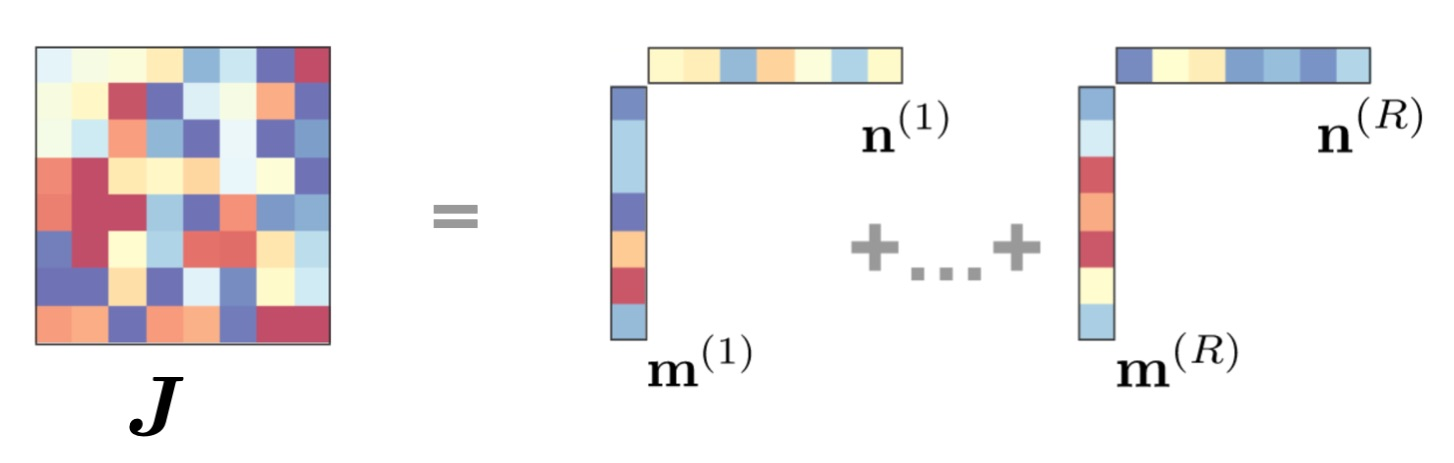
\includegraphics[width=0.6\textwidth]{../figures/low_rank_RNN_without_noise.jpg}
			\caption{\textbf{Low-rank recurrent networks (RNNs) constructed with distinct Gaussian distribution \cite{beiran2023parametric}}. A low-rank matrix could be written as a sum of outer products of vectors that are Gaussian distributed. As a result, the connectivity matrix is a mixture of Gaussians. }
			\label{fig:low_rank_RNN_without_noise}
		\end{figure}
	The connection matrix is constructed as a $n \times n$ dimensional matrix $J$ where $n$ is the number of neurons. Using singular value decomposition, the connectivity matrix with rank $G \ll n$ can be expressed as the sum of $G$ unit rank terms
		\begin{equation} \label{eq:low_rank_RNN_without_noise}
			J_{ij} = \frac{1}{n}\sum_{g = 1}^{G} l_i^{(g)}r_j^{(g)} \, \, \text{or} \, \, J = \frac{1}{n} \sum_{g=1}^{G} l^{(g)} r^{(g)T} \, . 
		\end{equation}
	The connectivity is therefore characterized by a set of $G$ $n$-dimensional vectors, or the $g$-th connectivity patterns, $l^{(g)} = \left\{l_i^{(g)}\right\}_{i = 1, ..., n } \in \mathbb{R}^{n \times 1}$ and $r^{(g)} = \left\{r_i^{(g)}\right\}_{i = 1, ..., n } \in \mathbb{R}^{n \times 1}$ for $g = 1, ..., G$. $\left\{l^{(g)}\right\}$ are the left singular vectors of the connectivity matrix and $\left\{r^{(g)}\right\}$ the right. The vectors $\left\{l^{(g)}\right\}$ and $\left\{r^{(g)}\right\}$ are mutually orthogonal and randomly multi-variate Gaussian distributed \cite{beiran2021shaping}. 
	
	\paragraph{Low-rank RNNs with random noise \cite{mastrogiuseppe2018linking}.}
	Similar to the construction of low-rank connection above (figure \ref{fig:low_rank_RNN_without_noise} defined by (\ref{eq:low_rank_RNN_without_noise})), \cite{mastrogiuseppe2018linking} suggested that the connectivity matrix can be constructed with a part $P$ to be fixed and known and a random uncorrelated part.
		\begin{figure} [H]
			\centering
			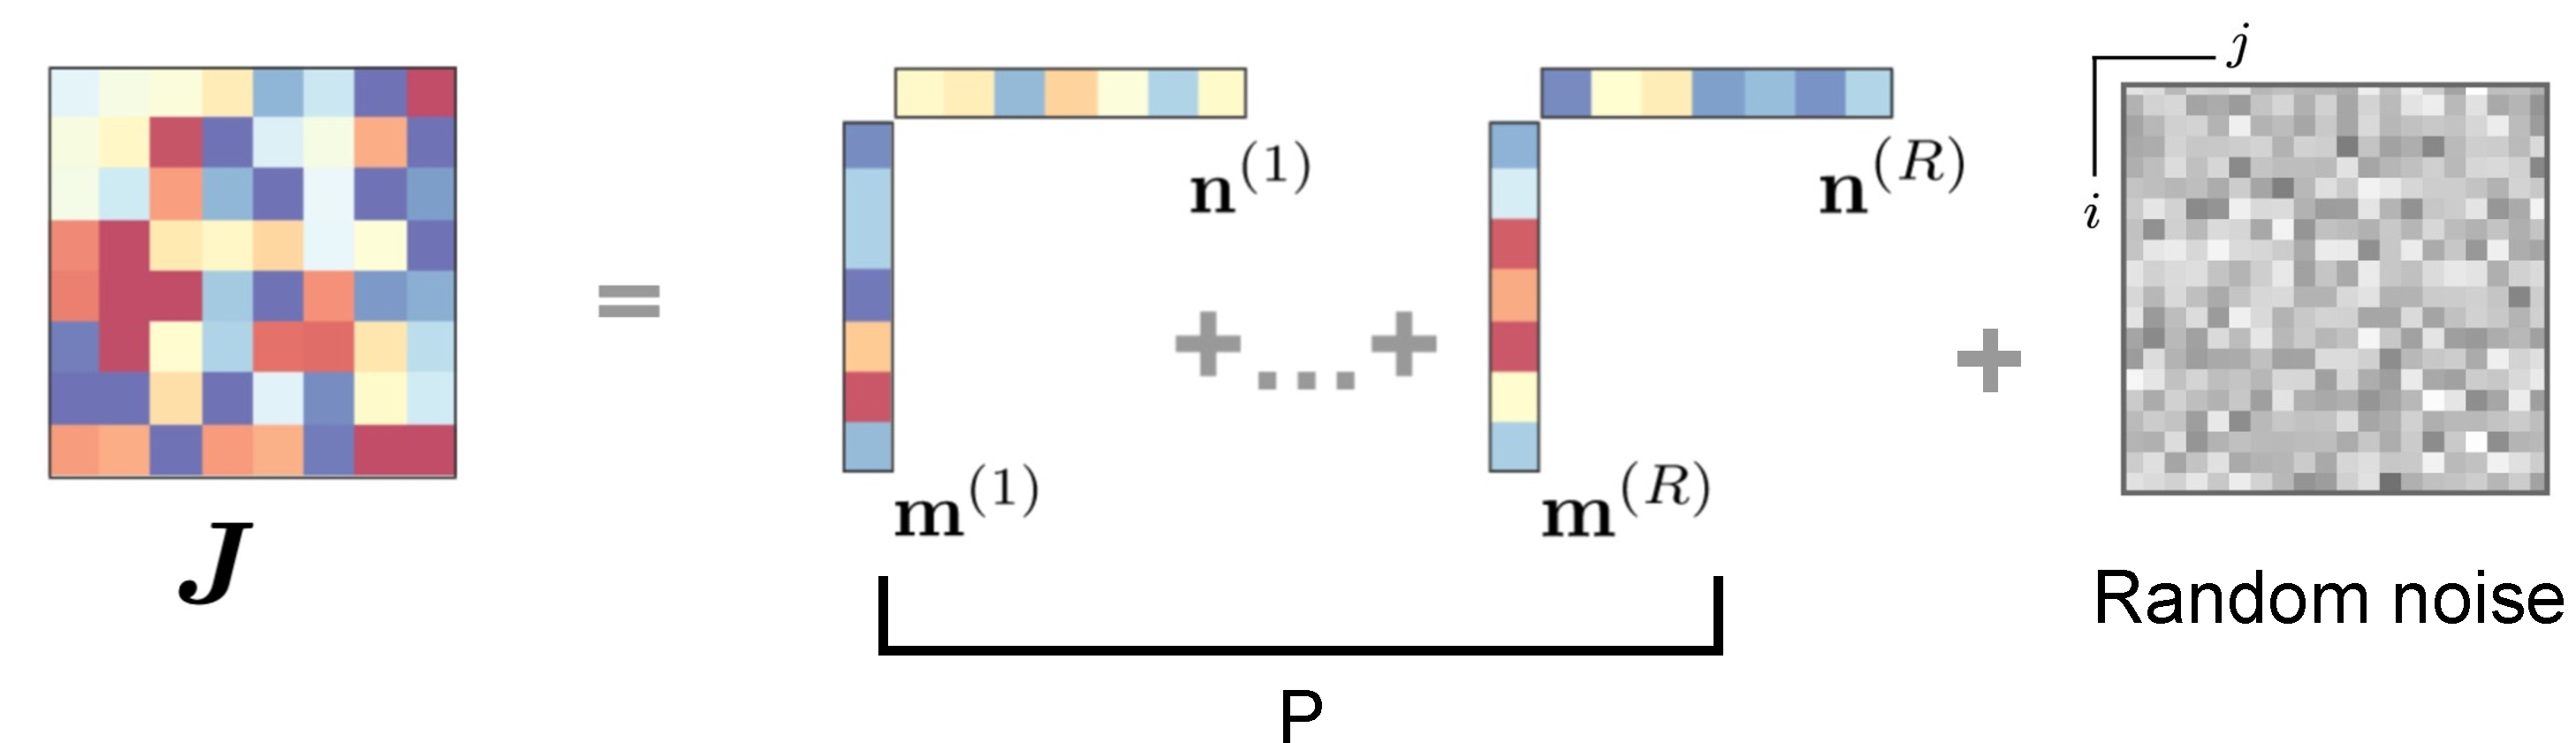
\includegraphics[width=0.75\textwidth]{../figures/low_rank_RNN_with_noise.pdf}
			\caption{\textbf{Low-rank recurrent networks (RNNs) constructed with fixed part and random noise \cite{mastrogiuseppe2018linking}.} The connectivity matrix is given by a sum of an uncontrolled, random matrix and a structured, controlled matrix $P$. Except for the fixed and know part $P$, which is a mixture of uncorrelated Gaussians, the RNN is disturbed by random noise.}
			\label{fig:low_rank_RNN_with_noise}
		\end{figure}
	The fixed part $P$ has the same construction as the network without noise (\ref{eq:low_rank_RNN_without_noise}). The uncontrolled random matrix can be constructed in a complex way with certain current-to-rate transfer function \cite{mastrogiuseppe2018linking}. 
	%For simplicity, we will try the random noise with a fully Gaussian distributed matrix. 
	That is
		\begin{equation} \label{eq:low_rank_with_noise}
			J = \frac{1}{n} \sum_{g=1}^{G} l^{(g)} r^{(g)T} + J_{\text{rand}} \, ,
		\end{equation}
	with $J_{\text{rand}}$ a $n \times n$ random matrix. 
	
	\subsubsection{Feedforward Recurrent Alignment Hypothesis with Low-rank RNNs} \label{sec:ffrec_low_rank}
	To test the feedforward recurrent alignmnent hypothesis applying the low-rank RNNs, we firstly consider the simple case of having symmetric low-rank connectivity, because symmetric structure is easier to interpret. Then we tried the asymmetric low-rank RNNs to discover the influence of rank on response properties. 
	
	\paragraph{Symmetric low-rank RNN}This could be achieved through choosing the left connectivity vectors $\left\{l^{(g)}\right\}$ equal the right connectivity vectors $\left\{r^{(g)}\right\}$. As a result the low-rank RNN without noise can be formulated by sum of symmetric matrices and therefore also symmetric:
		\begin{equation} \label{eq:sym_low_rank}
			J = \frac{1}{n}\sum_{g =1}^{G} l^{(g)} l^{(g)T} \, \, \text{or} \, \, J = \frac{1}{n}\sum_{g =1}^{G} r^{(g)} r^{(g)T} \, .
		\end{equation}
	If considering the connectivity matrix with noise, for simplicity, we add a random $n \times n$ symmetrized Gaussian distributed matrix to $J$ from (\ref{eq:sym_low_rank}).
	
	The dynamics and conditions for stable stability of the response in the symmetric low-rank RNNs should be kept the same as with symmetric full rank RNNs (\ref{eq:sym_response_ODE}, \ref{eq:sym_stable_fix_point}). In order to keep the steady state of responses stable, the eigenvalues $\lambda_i \in \mathbb{R}$ of the low-rank RNNs $J$ (\ref{eq:sym_low_rank}) are limited by $R < 1$ through normalizing with the maximal eigenvalue (\ref{eq:eigval_normal}). 
	
	\paragraph{Asymmetric low-rank RNN} When the set of left connectivity vector  $\left\{l^{(g)}\right\}$ is different from the set of right connectivity vector $\left\{r^{(g)}\right\}$, we receive the asymmetric low-rank with (\ref{eq:low_rank_RNN_without_noise}) for the case without random noise. If considering the random noise, we again add a simple $n \times n$ Gaussian distributed full rank asymmetric matrix as figure \ref{fig:low_rank_RNN_with_noise} illustrated (\ref{eq:low_rank_with_noise}). 
	
	To enable the stable steady state of responses, as shown in asymmetric RNNs (\ref{eq:asym_stable_fix_point}), the real part of eigenvalues $\text{Re}(\lambda_i)$ of asymmetric RNNs $J$ (\ref{eq:low_rank_with_noise}) are limited by $R < 1$ through normalization with the maximal magnitude of eigenvalues (\ref{eq:asym_normalization}). 
	
	\subsubsection{Evaluation of Feedforward Recurrent Alignment Hypothesis Based on Response Properties}
	Similar to the analysis on full rank networks, we also want to evaluate the modulation of feedforward recurrent alignment for low-rank RNNs based on the four response properties in correlation with feedforward recurrent alignment: 
		\begin{itemize}
			\item Trial-to-trial correlation
			\item Intra-trial stability
			\item Dimensionality 
			\item Alignment of evoked activity pattern to spontaneous activity pattern
		\end{itemize}
	
	\paragraph{Symmetric low-rank RNN} For symmetric low-rank RNN, the methods for modulations and evaluations are traced back to the full rank symmetric RNN before. The feedforward recurrent alignment is defined by (\ref{eq:ffrec_align}). Moreover, the trial-to-trial correlation is quantified with (\ref{eq:ttc_sym}), the intra-trial stability with (\ref{eq:its_sym}), the dimensionality with (\ref{eq:dim_analytical_sym}) and (\ref{eq:dim_empirical_sym}), and at the end the alignment to spontaneous activity with (\ref{eq:align_to_spont_act_sym}). 
	
	\paragraph{Asymmetric low-rank RNN} Since for asymmetric low-rank RNNs, the problem of complex eigenvectors and eigenvalues still exists, the modifications undertaken at asymmetric full rank RNNs (section \ref{sec:modify_ffrec_alignment_score} and \ref{sec:modification_asym}) can therefore be directly applied here, when align the inputs to the RNN. Generally, the modifications that were considered can be roughly described as: 1) only consider real part of eigenvalues and eigenvectors, 2) consider for each neuron the magnitude of inputs and variance ratio, 3) align the inputs to symmetrized network to approximate. 
	
	\clearpage
	\subsection{Black Box Recurrent Network Model}
	% Background
	Until now, we assume that we already know the structure of recurrent networks and evaluate the feedforward recurrent alignment hypothesis on the networks. However, in reality during the experiments, mostly only a small part of the network is known and the total structure of the network keeps mostly like a black box. As a result, the eigenvectors of the networks are generally unknown. The feedforward recurrent alignment cannot use the dominant modes to characterize the development of feedforward recurrent network system. 
	
	% Motivation from multiple experiments. Literatures
	It was pointed out that the reliability of evoked dynamics in recurrent networks is dependent on the stimulus used. As a consequence, to a recurrent network would correspond a set of stimuli which are more efficiently transmitted than others \cite{marre2009reliable}. 
	Especially the stimulus inputs that align with the structure of endogenous sub-networks would be recurrently amplified, leading to more reliable evoked responses \cite{mulholland2023selective}. 
	
	Besides, the similarity between spontaneous and evoked activity in sensory cortical areas could be a signature of efficient transmission and propagation across cortical networks. Based on a better recall caused by a match between spontaneous activity and input statistics, it was hypothesized that the recurrent connectivity could have been shaped by a learning process so that the spontaneous activity matches the natural input statistics \cite{marre2009reliable}. 
	
	% Explanation of the intuition. Want to approximate the dominant modes.
	Therefore, we wonder if we could apply the experimental measurable spontaneous activity to characterize the feedforward recurrent alignment. Without knowing the eigenvectors of the recurrent networks, align feedforward inputs to the spontaneous activity instead of the recurrent networks. This can be a further modification for modeling feedforward recurrent alignment for general asymmetric recurrent networks. 
	%TODO: connections between white noise and spontaneous activity --> H.Mulholland Lab see results. + difference between white noise evoked spontaneous-like activity (generating similar data) and spontaneous activity we modeled (fitting to ex.data).
	
	Furthermore, we consider to repeatedly apply the recurrently amplified spontaneous stimuli as inputs to discover if the amplified spontaneous activity could increase the alignment to the recurrent network. 
	
	\subsubsection{Approximation with White Noise Evoked Activity} \label{sec:white_noise_approx_ffrec}% Low rank is here not necessary (could perhaps shortly in Appendix).
	%TODO: distinguish the white noise evoked spontanous activity and modeled spontanous acttivity at alignment. Therefore from beginning change the sponatenous activity to white noise evoked ...
	% TODO: Connection between white noise evoked activity and spontaneous activity.
	With unknown recurrent structure, which we assume to be asymmetric generally, it is then difficult to find the stimuli pattern such that the trial-to-trial correlation, intra-trial stability and alignment between evoked activity to spontaneous activity to be high while keeping dimensionality low. In other words, we cannot apply the eigenvalues of the recurrent network to align with inputs and then characterize the development of feedforward inputs leading to stable response properties. 
	
	Alternatively, we align the inputs to spontaneous pattern and explore the response properties correlation with feedforward recurrent alignment. 
		
	% Definition of feedforward recurrent alignment with principal component.
	Spontaneous activity is evoked by white noise $h \in \mathbb{R}^{n \times 1}$, which is modulated by multivariate normal distribution with mean zero vector $0_v \in \mathbb{R}^{n \times 1}$ and covariance matrix the identity matrix $I_n \in \mathbb{R}^{n \times n}$, 
		\begin{equation}
			h_{\text{white}} \sim \mathcal{N}(0_v, I_n) \, .
		\end{equation}
	The spontaneous activity is then modeled by the transformed steady state response $r \in \mathbb{R}^{n \times 1}$, which is also multivariate normal distributed with transformed covariance matrix, 
		\begin{equation}
			r_{\text{white}} \sim \mathcal{N}\left(0_v, (1-J)^{-1}(1-J)^{-T}\right) \, .
		\end{equation}
	The response pattern is determined by the covariance matrix. If align the inputs to response patterns, the eigenvectors of covariance matrices are aligned. The eigenvectors of a covariance matrix are also known as principal components for the distribution. 
	
	To model the feedforward recurrent alignment hypothesis, the inputs are aligned to principal components and the feedforward alignment score is formulated with principal components instead of with modified eigenvectors of asymmetric recurrent network like section \ref{sec:modify_ffrec_alignment_score}. For a input $h$ aligned to a principal component $p$, the feedforward recurrent alignment is constructed with 
		\begin{equation} \label{eq:ffrec_white_noise}
			\nu := \frac{p^T J p}{\Vert p \Vert^2} \, .
		\end{equation}
	
	% Evaluation of the modification. monotony, ttc, its, dim, align to spont.act
	The original recurrent network is now approximated by the spontaneous response pattern and the inputs are aligned to principal components of the spontaneous response pattern. As for the recurrent networks, some properties of the new formulated feedforward recurrent alignment score have to be evaluated. The perspectives that we take into account are:
		\begin{itemize}
			\item Monotonously growing correlation between feedforward recurrent alignment score and eigenvalues of covariance matrix from spontaneous activity pattern.
			\item Positive correlation between feedforward recurrent alignment score and trial-to-trial correlation.
			\item Positive correlation between feedforward recurrent alignment score and intra-trial stability.
			\item Negative correlation between feedfroward recurrent alignment score and dimensionality.
			\item Feedforward recurrent alignment score is positive correlated with alignment of evoked activity to spontaneous activity.
		\end{itemize}
	
	% Monotony Method.
	\paragraph{Monotony} The feedforward recurrent alignment should reflect how well the input pattern is aligned with the considered recurrent network. The more the input pattern is aligned with the dominant projection direction in activity space, the stronger should be the evoked response due to response amplification. %TODO: should move the response amplification from results to introduction or method perhaps?.
	The response strength is determined by the corresponding eigenvalue of aligned direction. Since the inputs are aligned to the spontaneous activity pattern, the feedforward recurrent alignment should be monotonusly positive correlated with the eigenvalues of spontaneous activity pattern. 
	
	% ttc method.
	\paragraph{Trial-to-trial correlation} We consider the case of general asymmetric recurrent network from section \ref{sec:asym_recurrent_network} with formulation considering different grade of symmetry (\ref{eq:asym_interaction_matrix}). Thus, the modification is similar to section \ref{sec:modify_ffrec_alignment_score}. The input pattern $h$ is aligned to the principal component $p$ of the covariance matrix from spontaneous activity pattern and therefore modeled by
		\begin{equation}
			h \sim \mathcal{N}(p, \sigma_{\text{trial}I_n}) \, .
		\end{equation}
	The steady state response evoked by the inputs are transformed multivariate normal distribution
		\begin{equation}
			r \sim \mathcal{N}\left((1-J)^{-1}p, \sigma_{\text{trial}} (1-J)^{-1} (1-J)^{-T}\right) \, .
		\end{equation}
	The trial-to-trial correlation reflects the variation between different trials. It is again the average of pairwise Pearson correlation between response trials as defined by $\beta_s$ (\ref{eq:ttc_sym}). 
	
	% its method.
	\paragraph{Intra-trial stability} Intra-trial stability quantifies the variation inside one response trial evoked by input. One time-dependent input and evoked steady state response trial is approximated by Euler-Maruyama scheme \ref{eq:euler_maruyama}. The input pattern $h$ is aligned to principal components $p$ of activity pattern. Therefore, the mean vector for $h$ is the aligned principal component $p$. The input and evoked response are therefore formulated as
		\begin{subequations}
			\begin{align}
				\mathrm{d} h & = p \mathrm{dt} + \sigma_{\text{time}} \mathrm{d} W \\
				\mathrm{d} r & = (-r + J \cdot p) \mathrm{d}t + \sigma_{\text{time}} \mathrm{d} W \, .
			\end{align}
		\end{subequations}
	The intra-trial stability is the time average of delayed response correlation defined by (\ref{eq:input_distribution_dimensionality}). 
	
	% dim method
	\paragraph{Dimensionality} For modulation of change in dimensionality along alignment, the covariance matrix for input distribution is constructed as \ref{eq:Sigma_dim} but with principal components $p_i$ of spontaneous activity as an approximation to the eigenvectors of the original recurrent network.  
		\begin{equation}
			\Sigma^{\text{Dim}} := \sum_{i=L}^{L+M} \text{exp}\left(\frac{-2(i-L)}{\beta}\right) p_i p_i^T \, .
		\end{equation}
	The input and the evoked activity are modeled by multivariate normal distribution 
		\begin{subequations} \label{eq:dim_white_noise}
			\begin{align}
				h & \sim \mathcal{N}(0_v, \Sigma^{\text{Dim}}) \\
				r & \sim \mathcal{N}(0_v, (I_n - J)^{-1} \Sigma^{\text{Dim}} (I_n - J)^{-T}) \,.
			\end{align}
		\end{subequations}
	The effective dimensionality (\ref{eq:effective_dimensionality_analytical}) is approximated empirically by the eigenvalues of covariance matrix from spontaneous activity pattern (\ref{eq:dim_empirical_sym}). 
	
	% alignment to spont. act
	\paragraph{Alignment between evoked activity and spontaneous activity}  To grantee the spontaneous has a broader input than the evoked activity, the spontaneous activity here for alignment to evoked activity is constructed similar to (\ref{eq:dim_white_noise}) but with a higher dimensioality $\beta_{\text{spont}} > \beta$. For the formulation of covariance matrix for spontaneous activity, the principal components from white noise evoked activity pattern is used in (\ref{eq:Sigma_spont_asym}). 
		\begin{equation}
			\Sigma^{\text{spont}} := \sum_{i=L}^{M+1} \text{exp}\left(\frac{-2(i-1)}{\beta_{\text{spont}}}\right) p_i p_i^T \, .
		\end{equation}
	The spontaneous activity is then modeled by
		\begin{equation} \label{eq:spont_act_white_noise}
			r \sim \mathcal{N}(0_v, (I_n - J)^{-1} \Sigma^{\text{spont}} (I_n - J)^{-T}) \,. 
		\end{equation}
	The amount of overlap between evoked activity pattern (\ref{eq:dim_white_noise}b) and the principal components of spontaneous activity (\ref{eq:spont_act_white_noise}) quantifies the alignment (\ref{eq:align_to_spont_act_sym}). The average alignment over all $N$ evoked response trials is the final alignment score for alignment to spontaneous activity.
		\begin{equation}
			\gamma = \frac{1}{N} \left(\frac{r^T_{i} \cdot \Sigma^{\text{spont}} \cdot r_{i}}{\Vert r_{i} \Vert^2 \text{Tr}(\Sigma^{\text{spont}} )}\right)
		\end{equation}
	
	\subsubsection{Iterative Approximation with Low Dimensional Inputs} \label{sec:repeat_low_dim_inputs}
	Low dimensional inputs can be generated experimentally easier than high dimensional inputs %, while the high dimensional inputs are almost not possible to be generated. 
	So, we wonder if the feedforward recurrent alignment can also be adapted to represent the development and better alignment under the settings that, 1) only low dimensional inputs are offered and 2) the original recurrent network is asymmetric but unknown.
	
	To model the low dimensional input, random orthonormal basis vectors for construction of covariance matrix $e_i$ are obtained through Gram-Schmidt process. The same scheme as $\Sigma^{\text{Dim}}$ is applied, 
		\begin{equation}
			\Sigma_{\text{Low}} := \sum_{i=0}^{M} \text{exp}\left(\frac{-2(i-1)}{\beta_{\text{Low}}}\right) e_i e_i^T \, .
		\end{equation}
	Low dimensionality is realized by parameter $\beta_{\text{Low}}$, which should be smaller than it in $\Sigma^{\text{Dim}}$ and $\Sigma^{\text{spont}}$.
	
	The low dimensional inputs are then modeled as multivariate normal distribution with mean the zero vector $0_v \in \mathbb{R}^{n \times 1}$ and covariance matrix $\Sigma^{\text{Low}}$, 
		\begin{equation} \label{eq:low_dim_input_white_noise}
			h_{\text{Low}} \sim \mathcal{N}(0_v, \Sigma_{\text{Low}}) \, .
		\end{equation}
	The response evoked by low dimensional input (\ref{eq:low_dim_input_white_noise}) is the linearly transformed multivariate normal distribution
		\begin{equation}
			r_0 \sim \mathcal{N}\left( 0_v, (1-J)^{-1} \Sigma_{\text{Low}} (1-J)^{-T} \right) \, .
		\end{equation}
	At this step, the feedforward recurrent alignment $\nu$ can be calculated with low dimensional input $h$ 
		\begin{equation} \label{eq:repeat_low_dim_ffrec}
			\nu_0 = \frac{h^T J h}{\Vert h \Vert^2} \,.
		\end{equation} 
	
	Prior knowledge predicts stimulus inputs that align to spontaneous activity can be recurrently amplified and lead to more reliable responses \cite{mulholland2023selective}. 
	%Besides, the recurrent connectivity pattern shapes so that the inputs matches better with spontaneous activity during development \cite{marre2009reliable}. the response can be better aligned with the spontaneous activity than the input 
	%TODO: briding the idea of repeatly applying the response.
	We therefore wonder if the responses also align better with the recurrent network and if the repeated apply of responses lead to a development of alignment to recurrent network. In other words, if the alignment of responses could also capture the neural development process in a certain way.
	
	For that, we apply repeatedly the prior response as the input for the network and at the same time update step wise the corresponding feedforward recurrent alignment. 
	
	If $r_0$ is the input for the recurrent network, the evoked response $r_1$ is due to the linear transformation of normal distribution also a multivariate normal distribution with linearly transformed variance.
		\begin{equation}
			r_1 \sim \mathcal{N}\left(0_v, \left((1-J)^{-1}\right)^2 \Sigma_{\text{Low}} \left((1-J)^{-T}\right)^2\right) \, .
		\end{equation}
	The corresponding feedforward recurrent alignment, noted as $\nu_1$, is determined by the input $r_0$,
		\begin{equation}
			\nu_1 = \frac{r_0^T J r_0}{\Vert r_0 \Vert^2}\, .
		\end{equation}
	Iteratively, at the $n$-th time of applying prior response $r_{n-1}$ as input, the evoked response $r_n$ has the general formulation of a multivariate normal distribution with linearly transformed covariance matrix,
		\begin{equation}
			r_n \sim \mathcal{N}\left( 0_v, \left((1-J)^{-1}\right)^{n+1} \Sigma_{\text{Low}} \left((1-J)^{-T}\right)^{n+1} \right) \,. 
		\end{equation}
	The corresponding $n$-th feedforward recurrent $\nu_n$ alignment has the general formulation with $r_{n-1}$,
		\begin{equation} \label{eq:update_ffrec}
			\nu_n = \frac{r_{n-1}^T J r_{n-1}}{\Vert r_{n-1} \Vert^2} \,.
		\end{equation}
	
	
	\clearpage
	\subsection{Hebbian Learning in Feedforward Recurrent Networks}
	% Following the iterative approximation from the last section. Motivation. The goal.
	In the neocortex, which forms the convoluted outer surface of the human brain, neurons lie in six vertical layers highly coupled within cylindrical columns. Feedforward connections bring input to a given region from another region located at an earlier stage along a particular processing pathway. Recurrent synapses interconnect neurons within a particular region that are considered to be at the same stage along the processing pathway \cite{dayan2005theoretical}. 
	
	Until now, we only considered the recurrent layer under given feedforward inputs (figure \ref{fig:symmetric_RNN}b and figure \ref{fig:asymmetric_RNN}b). However, the feedforward inputs are also the outputs from feedforward network. In this part of work, we will expand the network structure to feedforward recurrent network containing input layer, feedforward interaction and output layer connected by recurrent interactions.
	
		\begin{figure}[H]
			\centering
			\includegraphics[width=0.5\textwidth]{../figures/feedforward_recurrent.pdf}
			\caption{\textbf{Illustration of a general feedforward recurrent network construction.} Shown in the figure is a feedforward recurrent network with input layer, output layer, a feedforward synaptic weight matrix for feedforward interactions, and a recurrent synaptic weight matrix for recurrent interactions. Firing rate models are applied in both input layer and output layer for modeling.}
			\label{fig:feedforward_recurrent_network}
		\end{figure} 
	
	% Hebbian Learning and plasiticity.
	Activity-dependent synaptic plasticity is widely believed to be the basic phenomenon underling learning and memory, and it is also thought to play a crucial role in the development of neural circuits \cite{dayan2005theoretical}. To count in this essential characteristic of networks during the development, we integrate the plasticity in the network dynamic. 
	
	The fundamental rule for synaptic plasticity in learning and memory is called the Hebb rule, raised by Donald Hebb in 1949. Hebb suggested that if input from neuron A often contributes to the firing of neuron B, then the synapse from A to B should be strengthened. In other words, neuron that fire together, wire together. The activity-dependent synaptic plasticity of the Hebbian type refers to the plasticity that is based on correlation of pre- and postsynaptic firing \cite{dayan2005theoretical}. 
	
	There are different types of training procedures for Hebbian type plasticity, including unsupervised learning, supervised learning, reinforcement learning, and so on. we mainly focus on the unsupervised learning. Unsupervised learning provides a model for the effects of experience on mature networks \cite{dayan2005theoretical}. Based on our network model (figure \ref{feedforward_recurrent_network}), we consider the case in which there are multiple postsynaptic neurons. 
	
	\subsubsection{Model Setting}
	% One input neuron model. Figure for the model construction. 
	To relief the understanding of dynamics during the modeling, we start with the simplified assumption of random symmetric recurrent interaction $J$ and linear feedfroward recurrent networks.
	
	Two basis cases are considered for our start up modeling: 1) only one input rate $u$, and 2) only Hebbian learning update of feedforward interaction $W$. The output layer keeps occupied by number of $n$ output neurons. 
	
	The feedforward interaction $W$ can be described as a $\mathbb{R}^{n \times 1}$ dimensional vector containing $W_i$ the strength of connection between $i$-th output neuron and input neuron. Output rates $v \in \mathbb{R}^{n \times 1}$ describes the activity firing rate for output neurons. The random symmetric interaction $J \in \mathbb{R}^{n \times n}$ is constructed in the same way as for feedforward recurrent alignment hypothesis in section \ref{sec:symmetric_recurrent_interaction}. 
	
		\begin{figure}[H]
			\centering
			\includegraphics[width=0.5\textwidth]{../figures/single_neuron_feedforward_recurrent.pdf}
			\caption{\textbf{Illustration of feedforward recurrent network model with single input neuron.} For start up of feedforward recurrent network dynamic analysis, the simple case of only one input neuron with fixed random symmetric recurrent interaction $J$. The output layer has number of $n$ neurons. The feedforward interaction matrix is updated with Hebbian rules.}
			\label{fig:single_neuron_feedforward_recurrent_network}
		\end{figure}
	
	The output rates $v \in \mathbb{R}^{n \times 1}$ in this linear case is determined by 
		\begin{equation} \label{eq:response_ffrec_network}
			\tau \frac{dv}{dt} = -v + W \cdot u + J \cdot v \,.
		\end{equation}
	For simplicity, the time scale constant is set to be $1$. The feedforward input is summarized by the part $h := W \cdot u \in \mathbb{R}^{n \times 1}$.  
	
	Provided that the real parts of the eigenvalues of $J$ are less than $1$, this equation has a stable fixed point with a steady-state output activity vector determined by (shown in section \ref{sec:steady_state_response_sym} and \ref{sec:asym_recurrent_network})
		\begin{equation} \label{eq:steady_eq_ffrec}
			v = W \cdot u + J \cdot v \, .
		\end{equation}
	Solving the above equation (\ref{eq:steady_eq_ffrec}), the steady state response for the feedforward recurrent network is
		\begin{equation} \label{eq:steady_state_ffrec}
			v^* = (I_n - J)^{-1} \cdot W \cdot u \, .
		\end{equation}
	
	\subsubsection{Update Rules for Feedforward Network}
	% The Differential equations for the update rules.
	For multiple postsynaptic neurons with fixed recurrent weights $J \in \mathbb{R}^{n \times n}$ and plastic feedforward weights $W \in \mathbb{R}^{n \times 1}$, the basic Hebbian modification over the training input $u \in \mathbb{R}$ is 
		\begin{equation} \label{eq:basic_Hebb}
			\tau_w \frac{dW}{dt} = vu \, , 
		\end{equation}
	where $\tau_w$ is a time constant that controls the rate at which the weights change and for simplicity set to be $1$. If and only if both presynaptic rate $u$ and postsynaptic rate $v$ has the same signs in rates, meaning that both pre- and postsynaptic activies are both suppressed or activated at the same time, the connection weight between those two neurons increases. Therefore, the equation (\ref{eq:basic_Hebb}) implies that simultaneous pre- and postsynaptic activity increases the feedforward synaptic strength.
	
	To compute the weight changes induced by a series of input patterns $u$, a convenient alternative is to average over all of the different input patterns and compute the weight change induced by this average, leading to the average Hebbian rule:
		\begin{equation} \label{eq:average_Hebb}
			\frac{dW}{dt} = \langle vu \rangle \, ,
		\end{equation}
	with angle brackets $\langle \, \rangle$ denoting averages over the ensemble of input patterns presented during training. 
	
	Replace the output rate $v$ in equation (\ref{eq:average_Hebb}) with the steady state formulation (\ref{eq:steady_state_ffrec}), the average plasticity rule can be rewrote as 
		\begin{equation}
			\frac{dW}{dt} = \langle (I_n - J)^{-1} \cdot W \cdot u u \rangle = (I_n - J)^{-1} \cdot W \cdot \langle uu \rangle \, .
		\end{equation}
	Defining $Q := \langle uu \rangle$ the input autocorrelation, the final formulation of average rule is
		\begin{equation}
			\frac{dW}{dt} = (I_n - J)^{-1} \cdot W \cdot Q \, .
		\end{equation}
	Since for the simple case here that $u \in \mathbb{R}$, the input autocorrelation $Q = 1$ for all input patterns. Therefore, specifically for the simple network (figure \ref{fig:single_neuron_feedforward_recurrent_network}) we consider, the average rule can be further written as
		\begin{equation} \label{eq:final_hebb_ff_weight}
			\frac{dW}{dt} = (I_n - J)^{-1} \cdot W \, .
		\end{equation} 

	\subsubsection{Projection of the Feedforward Weights on Eigenvectors}
	% What do the projects and how the projects are calculated.
	With the average Hebbian rule, the dynamic of the feedforward weight $W$ can be approximated with the help of Euler scheme, resulting the iterative update for $W$ at time point $t+1$
		\begin{equation} \label{eq:euler_scheme_ffrec_weight}
			W_{t+1} = W_t + \Delta t (I_n - J)^{-1} \cdot W_t \, , 
		\end{equation}
	where $\Delta t$ is a enough small time distance during the total time period $T$. The initial weight $W_0$ for iteration is random Gaussian distributed.
	
	As a result, the change of connections between each output neuron and the single input neuron over time can be approximated through equation (\ref{eq:euler_scheme_ffrec_weight}). The distribution of the weights can be an important information about which connections are strengthened over time by unsupervised learning of feedforward interaction. 
	
	% Introduce the idea and perpose for projections. 
	Moreover, the output from feedforward interaction $h := W \cdot u$ is exactly the feedforward input for the recurrent interaction.  Continuing the idea from feedforward recurrent alignment hypothesis, align the feedforward input $h$ well to recurrent network could predict the reliability of evoked activity. Since $u \in \mathbb{R}$, the feedforward input for recurrent network is proportional to the feedforward weight vector $W$. Therefore, we align the feedforward weight vector $W$ to recurrent network through projection of vector $W$ to space spanned by eigenvectors of recurrent network. 
	
	Recurrent network has symmetric interaction $J$, thus the eigenvectors $\{e_i\}_{i = 1, ..., n}$ of $J$ is a set of basis vectors that span the vector space $\mathbb{R}^n$. The feedforward weight vector $W \in \mathbb{R}^{n \times 1}$ can be expressed as linear combination of eigenvectors $\{e_i\}$. For better interpretation, $\{e_i\}$ are ordered so that their corresponding eigenvalues $\{\lambda_i\}$ are in descending order:
		\begin{equation}
			e_{\text{max}}, ..., e_i, e_j, ..., e_{\text{min}} \, \, \text{such that} \, \, \lambda_{\text{max}} > ...> \lambda_i > \lambda_j > ... > \lambda_{\text{min}} \, .
		\end{equation} 
	The feedforward weight vector $W_t$ at time point $t$ can be formulated as
		\begin{equation} \label{eq:linear_combi_weight}
			W_t = \sum_{i = 1}^{n} \phi_i e_i = A \phi \, ,
		\end{equation}
	where $\phi \in \mathbb{R}^{n \times 1}$ is the vector containing all projection coefficients $\phi_i$ and $A$ is the matrix containing the eigenvectors $e_i$ column wise.  
	
	As a result, the projection coefficient can be gained through equivalent reformulation of equation (\ref{eq:linear_combi_weight}), 
		\begin{equation} \label{eq:calculation_ratio}
			\phi = A^{-1} \cdot W_t \, .
		\end{equation}
	Matrix $A$ is invertible because all columns of $A$ are linearly independent. 
	
	The distribution of $\phi_i$ reflects to which eigenvectors directions the feedforward weight vector $W$ and thus also the feedforward input $h$ aligns to the recurrent network more or less. According to the feedforward recurrent alignment hypothesis, in experienced feedforward recurrent network, the feedforward input align to the dominant eigenvectors of recurrent interaction matrix, those are the eigenvectors with large eigenvalues. Alignment to dominant eigenvectors can be reflected by the projection coefficients for them. 
	
	To more directly quantify the change of alignment of $W$ to dominant eigenvectors, we define the projection ratio $\rho$ as the percentage that the coefficients for the first twenty eigenvectors \footnote{Under the initial condition that the number of neurons $n$ is larger than $20$. } over all coefficients. Since the sign of coefficients only reflects the direction of alignment, we consider the absolute number for calculation of projection ratio $\rho$.
		\begin{equation} \label{eq:projection_ratio}
			\rho := \frac{\sum_{i=1}^{20} \vert \phi_i \vert}{\sum_{i=1}^{n} \vert \phi_i \vert} \, .
		\end{equation}
		
	\subsubsection{Dynamics of Feedforward Recurrent Alignment}
	% The derivative of feedforward recurrent alignment with update of feedforward weight. 
	% Development and the derivative of the feedforward recurrent alignment.
	
	An alternative to discover the feedforward recurrent alignment hypothesis is to directly observe the dynamic of feedforward recurrent alignment score in the network. With the time dependent update of feedforward weight vector $W$ by Euler-scheme equation (\ref{eq:euler_scheme_ffrec_weight}), the feedforward input for recurrent network $h$ can be updated simultaneously through multiplying input rate $u$, 
		\begin{equation} \label{eq:feedforward_input}
			h_t = W_t \cdot u_t \, ,
		\end{equation}
	with $h_t,\, W_t, \, u_t$ the feedforward input for recurrent network, feedforward interaction, and input at time point $t$. 
	
	The develop of feedforward recurrent alignment score over time can be then calculated with its definition inserting the updated feedforward input for recurrent network $h_t$. The feedforward recurrent at time point would be $\nu_t$ with
		\begin{equation} \label{eq:ffrec_update}
			\nu_t = \frac{h_t^T J h_t}{\Vert h_t \Vert ^2} = \frac{u_t W_t^T J W_t u_t}{u_t^2 \Vert W_t \Vert ^2} = \frac{W_t^T J W_t}{\Vert W_t \Vert^2}\, . 
		\end{equation}
	Because $u_t \in \mathbb{R}$ for all $t$, the feedforward recurrent alignment $\nu_t$ is directly determined by feedforward weight vector $W_t$.  
	
	The derivative of feedforward recurrent alignment $\nu_t$ can illustrate the change over time more intuitively. For further calculation, calculating firstly the derivative of numerator and denominator of $\nu_t$ in equation (\ref{eq:ffrec_update}). Defining thereby the numerator as $g(t)$ and denominator $h(t)$. Without loss of generality, the Euclidean norm is applied for denominator. That is
		\begin{subequations}
			\begin{align}
				g(t) &:= W_t^T J W_t\\
				h(t) &:= \Vert W_t \Vert_2^2
			\end{align}
		\end{subequations}
	Applying product rule for derivative of $g(t)$ and chain rule for $h(t)$, it results in
		\begin{equation}
				\frac{\mathrm{d}g(t)}{\mathrm{d}t} = \frac{\mathrm{d}W_t^T}{\mathrm{d}t} J W_t + W_t^T J \frac{\mathrm{d}W_t}{dt} \, .
		\end{equation}
	Inserting the Hebbian rule (\ref{eq:final_hebb_ff_weight}) for feedforward weights leads to
		\begin{equation}
			\frac{\mathrm{d}g(t)}{\mathrm{d}t} = W_t^T (I_n - J)^{-T}J W_t + W_t^T J(I_n - J)^{-1} W_t \, .
		\end{equation}
	Since the recurrent network interaction $J$ is symmetric, the matrix $(I_n-J)$ and its inverse matrix is also symmetric. Therefore, $(I_n - J)^{-T} = (I_n - J)^{-1}$. So, the final derivative of numerator $g(t)$ is
		\begin{equation}
			\frac{\mathrm{d}g(t)}{\mathrm{d}t} = W_t^T \left( (I_n - J)^{-1}J + J(I_n - J)^{-1}\right)W_t \, .
		\end{equation}
	
	The derivative of denominator can be obtained after inserting the Euclidean norm 
		\begin{equation}
			\begin{split}
				\frac{\mathrm{d}h(t)}{\mathrm{d}t} & = \frac{\mathrm{d} \Vert W_t \Vert_2^2}{\mathrm{d}t} = \frac{\mathrm{d} \sum_{i=1}^{n} W_{t, i}^2}{\mathrm{d}t}
				= \sum_{i=1}^{n} \frac{\mathrm{d}W_{t,i}^2}{\mathrm{d}t} = 2W_t^T \frac{\mathrm{d}W_t}{\mathrm{d}t} \\
				& = 2W_t^T (I_n - J)^{-1} W_t \,.
			\end{split}
		\end{equation}
	The last equation is due to the Hebbian rule differential equation (\ref{eq:final_hebb_ff_weight}). 
	
	Following the quotient rule with derivatives of numerator $g(t)$ and denominator $h(t)$, the derivative for feedforward recurrent alignment score is 
		\begin{equation}
			\begin{split}
				\frac{\mathrm{d}\nu_t}{\mathrm{d}t} &= \frac{\frac{\mathrm{d}g(t)}{\mathrm{d}t}h(t) - g(t)\frac{\mathrm{d}h(t)}{\mathrm{d}t}}{h(t)^2} \\
				&= \frac{W_t^T \left( (I_n - J)^{-1}J + J(I_n - J)^{-1}\right)W_t \Vert W_t \Vert_2^2 - 2W_t^TJW_tW_t^T (I_n - J)^{-1} W_t }{\Vert W_t \Vert_2^4} \\
				&= \frac{W_t^T}{\Vert W_t \Vert_2} (I_n-J)^{-1} J \frac{W_t}{\Vert W_t \Vert_2} + \frac{W_t^T}{\Vert W_t \Vert_2} J (I_n-J)^{-1} \frac{W_t}{\Vert W_t \Vert_2} \\
				&\, \, \, \, \, \, \, \, \, -2 \frac{W_t^T}{\Vert W_t \Vert_2} J \frac{W_t}{\Vert W_t \Vert_2} \frac{W_t^T}{\Vert W_t \Vert_2} (I_n-J)^{-1} \frac{W_t}{\Vert W_t \Vert_2}  \, .
			\end{split}
		\end{equation}
	To simplify the notation, defining the normalized feedforward weights as $\bar{W_t}$. Thus, the final formulation of the derivative for feedforward recurrent alignment score at time point $t$ is
		\begin{equation} \label{eq:derivative_ffrec}
			\frac{\mathrm{d}\nu_t}{\mathrm{d}t} = \bar{W_t}^T (I_n-J)^{-1}J\bar{W_t} + \bar{W_t}^T J(I_n -J)^{-1} \bar{W_t} - 2\bar{W_t}^TJ\bar{W_t}\bar{W_t}^T(I_n-J)^{-1}\bar{W_t} \, .
		\end{equation}
	
	
	
\end{document}